\documentclass[main.tex]{subfiles}
\begin{document}

% \marginpar{Friday\\ 2019-11-15, \\ compiled \\ \today}
% \section*{Fri Nov 15 2019}

% We start again from where we left off, with hydrogen recombination.

% We want to estimate the moment at which hydrogen first formed, which marks the point at which electrons and photons interact efficently: before, they interacted with Compton scattering which is very efficient; after they interact with hydrogen atoms in a way that is very inefficient.

% After this, then, we say that photons and matter are \emph{decoupled}.

% The scattering cross section (for Compton?) goes like the inverse square of the mass.

% This means that the universe is not only \emph{globally},  but also \emph{locally} neutral.

% This decoupling is what allows for star formation.
% Also, this is when the CMB starts.
% It is made of microwaves now, but it was higher earlier.

% The phase space distribution of photons is scale-invariant since they have zero mass: so we can say that the photons' distribution \emph{looks} thermal, but it is actually not technically since there are no interactions anymore.

% However the photons travel freely and are perceived as thermal, and they give an almost perfect blackbody! The errorbars in a plot for it must be magnified by \num{e4} in order to be seen.

% Neutrality implies \(n_e = n_p\).
Let us now introduce the total baryon density, \(n_b\).
In principle, we should account for Helium: as we will see, a couple of minutes after the Big Bang He-4 nuclei started to form, but they made up only something like \(25\%\) of the mass, which means \(6\%\) of the number density: so we ignore them and say that the number density of baryons is 
%
\begin{align}
  n_b = n_p + n_H
\,.
\end{align}

% Our ansatz for the Boltzmann equation is \(\mu_e + \mu _p = \mu _H\) since photons have no chemical potential.

% \(i\) denotes a generic one in \(e\), \(p\) and \(H\).
% Then 
% %
% \begin{align}
%   n_i = g_i\qty(\frac{m_i T}{2 \pi })^{3/2} \exp(\frac{\mu _i - m_i}{T})
% \,,
% \end{align}
% %
% we need to account for the chemical potential since it is the driver of this process.
The quantity we want to describe is how much hydrogen is still ionized: this is given by the ratio of the free electrons to the total baryons, \(n_e / n_b\). This is called the \textbf{ionization fraction} \(X_e\), and is also equal to \(n_p / n_b\) since the universe must be globally neutral. 

We expect to have \(X_e = 1\) in the early universe, and \(X_e = 0\) after the end of reionization.

This is a good model to keep in mind although it is not precisely correct, since simulations show that there will be some \emph{residual ionization}: \(X_e\) only goes to around \(\num{e-4} \divisionsymbol \num{e-5}\) at the end of reionization.
Also, in the modern universe a large fraction of the hydrogen has become ionized again, especially in the intergalactic medium; this is likely due to the energy injected into it by structure formation, which definitely breaks the approximation of global thermal and chemical equilibrium. 
This is not a concern for us: here, we only wish to describe the processes in the interval \(1000 \lesssim z \lesssim 2000\). 
 
%  naively we'd expect it to get to 0, but actually there remains some residual ionization, some free protons and electrons.
% How much is \(n_e / n_b\)? the same as \(n_p / n_b\). We call this quantity \(X_e\), the ionization number.
% A proper calculation would account for the non-equilibrium contributions.
% However, we estimate the process as being in equilibrium: this will underestimate the number of electrons.

% Today, most of the hydrogen is ionized (there is a ***-Peterson effect which shows this): this means that matter and radiation interact again.

% This is the second important time in the history of the universe.

% Can we see the early stars? Not really, we see galaxies only up to \(z \sim 10\), these stars would be at something like \(z \sim 30\)\dots
% There might be more to this.

% Inserting this and the Saha equation we get
% So the number density of hydrogen atoms is given by: 
%
% \begin{align}
%   n_H = g_H \qty(\frac{m_H T}{2 \pi })^{3/2} \exp(\frac{\mu_p - \mu_e - m_p - m_e + B}{T})
% \,,
% \end{align}
%
% and we can simplify things since \(m_p, m_H \gg m_e, B\), and substitute in the number densities for electrons and protons.
The binding energy of the hydrogen is \(B=m_p+m_e-m_H=\SI{13.6}{eV}\), so instead of \(m_H\) we can write \(m_H = m_p+m_e-B\).
Let us insert this expression and the Saha equation in the expression for the hydrogen number density; then we will recognize part of the expressions for the proton and electron number densities, which we can 
%
\begin{subequations}
\begin{align}
  n_H &=  g_H \qty(\frac{m_H T}{2 \pi })^{3/2} \exp(\frac{\mu _H - m_H}{T})  \\
  &= g_H \qty(\frac{m_H T}{2 \pi })^{3/2} \exp(\frac{\mu_e + \mu _p - m_e - m_p + B}{T}) \\
  &= \underbrace{\frac{g_H}{g_e g_p}}_{= 1} \cancelto{}{\qty(\frac{m_H T}{2 \pi })^{3/2}}
  \qty(\frac{m_e T}{2 \pi })^{-3/2}
  \cancelto{}{\qty(\frac{m_p T}{2 \pi })^{-3/2}}
  n_e n_p
  \exp(\frac{B}{T}) \\
  \frac{n_H}{n_e n_p} &=  \qty(\frac{m_e T}{2 \pi })^{-3/2} \exp(\frac{B}{T})  \\
  \frac{n_b - n_p}{n_p^2} &= \qty(\frac{m_e T}{2 \pi })^{-3/2} \exp(\frac{B}{T}) 
\,,
\end{align}
\end{subequations}
%
which we can manipulate, using the following identity: 
%
\begin{align}
  \frac{n_b - n_p}{n_p^2} = \frac{n_b \qty(1 - n_p/ n_b)}{n_b^2 X_e^2} = \frac{1}{n_b} \frac{1 - X_e}{X_e^2}
\,,
\end{align}
%
where we use \(n_e = n_p\) and the definition of \(X_e = n_p / n_b\). Then, we bring the \(n_b\) to the other side of the equation and multiply and divide by the photon number density, which is given by
%
\begin{align} \label{eq:n-gamma}
  n_{\gamma } = \frac{2 \zeta (3) T^3}{\pi^2}
\,.
\end{align}

With this, we can insert the baryon fraction \(\eta_b\) (which is conserved, so we can use its current value):
%
\begin{subequations}
\begin{align}
  \frac{1- X_e}{X_e^2} &= \underbrace{\frac{n_b}{n_\gamma }}_{\eta_p} 
  n_\gamma
  \qty(\frac{m_e T}{2 \pi })^{-3/2} \exp(\frac{B}{T})   \\
  &= \eta_0 \frac{2 \zeta (3)T^3}{\pi^2} \qty(\frac{m_e T}{2 \pi })^{-3/2} \exp(\frac{B}{T})   \\
  &= \eta_0  \frac{4 \sqrt{2} \zeta (3)}{\sqrt{\pi }} \qty(\frac{T}{m_e})^{3/2} \exp(\frac{B}{T}) \label{eq:saha-equation-ionization}
\,,
\end{align}
\end{subequations}
%
which we can solve numerically to find \(X_e\) as a function of temperature, or of redshift. The results are shown in figure \ref{fig:ionization}. 

\begin{figure}[ht]
\centering
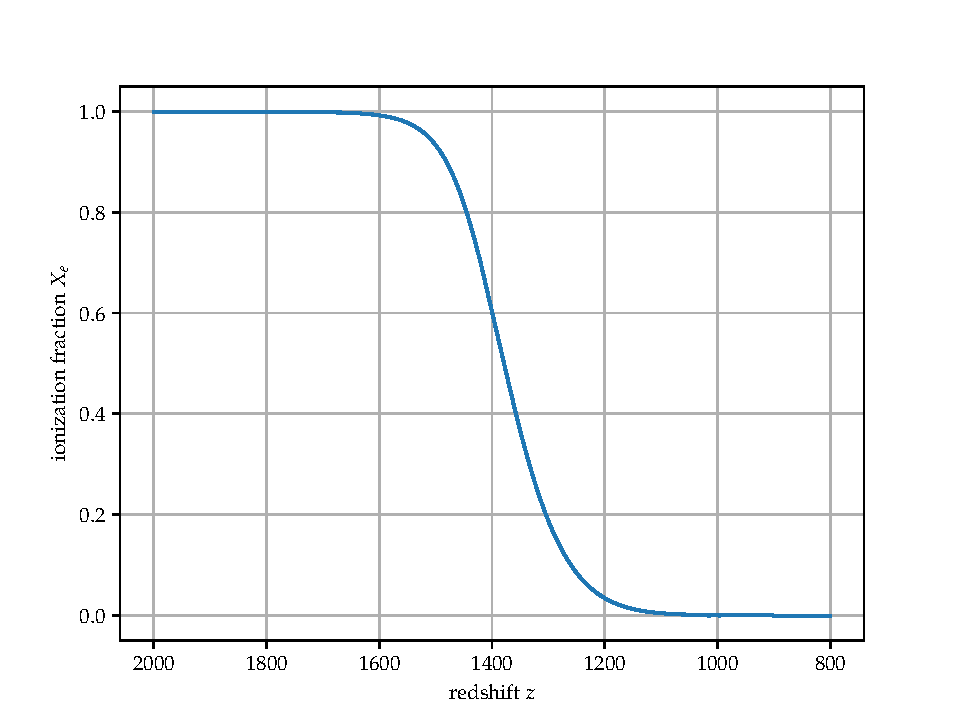
\includegraphics[width=\textwidth]{figures/ionization}
\caption{Ionization fraction as a function of redshift: a numerical solution of equation \eqref{eq:saha-equation-ionization}.}
\label{fig:ionization}
\end{figure}

Let us try to understand what is going on. Roughly speaking, we get intermediate values for \(X_e\), like \(\num{.5}\), when the right-hand side is of order 1.
If the right-hand side only contained the terms \((T/m_e)^{3/2}\exp(B/T)\) without any multiplicative factor in front (meaning, roughly, that we had \(\eta_0 \sim 1\)), then we would see recombination starting to occur already at \(z \sim 4000\) (\(T \sim \SI{1}{eV}\)), and by \(z \sim 2000\) if would almost be over.
The reason this does not happen is that \(\eta_0 \) is \emph{very small}: there are a lot of photons, many more than the baryons, which are ready to dissociate any atoms which start to form.

So, hydrogen is truly formed only when \(T \sim \SI{0.3}{eV}\), much lower than its ionization energy.

\todo[inline]{But even with \(\eta_0 \sim 1\) we get formation at \(T \sim \SI{1}{eV}\), an order of magnitude less than \(B\)! is there an intuitive argument as to why this is the case?}

The estimates we gave do depend on the value we assign to \(\Omega_{0b}\) and \(h\), however within the currently accepted experimental ranges the main predictions do not vary substantially. 

% Approximately, it occurred somewhere around \(z \sim 1100\) (we conventionally say that recombination happened when \(X_e = 0.1\)).
The process of recombination is gradual, but we can choose a conventional redshift as, for example, the time when we reach an arbitrary threshold like \(X_e = \num{.1}\). 

The interaction rate between photons and free electrons is \(\Gamma_{\gamma } = n_e \sigma_T c\), where \(\sigma _T\) is the Thompson cross section while \(n_e\) is the number density of free electrons, which can be estimated as \(n_e = n_b X_e \approx \rho_C \Omega_{b} X_e / m_p\). 
% After recombination, we have the \emph{last scattering}: the moment at which the CMB was formed.
Then, we can estimate the moment of the last scattering by checking the decoupling condition: \(\Gamma _\gamma < H\). 
With the numbers given earlier, we find \(z \sim 1120\): a very good approximation to the currently accepted value \(z \sim 1089\)!

% One Nobel prize this year was awarded to Jim Peebles, a friend of Sabino's: together with his PhD supervisor Dicke, he was the first to calculate this stuff.

% Peebles in 1964 (?) did this calculation both in GR and in Brahms-Dicke theory, a modified gravity theory.

\todo[inline]{Then Pacciani has an argument as to why \(T \sim a^{-2}\) for matter, should this be included here?}

\section{Primordial nucleosynthesis}

Already in the 1940s it was noticed by Alpher, Bethe as well as Gamow that the abundances of certain nuclides could not be explained if they were formed in stellar interiors alone. 
Specifically, the issue is with the abundances of light elements: deuterium \(\ce{^{2}H}\), as well as \(\ce{^{3}He}\) and \(\ce{^{4}He}\), while heavier nuclides (with mass number \(A \geq 7\)) could not form in the early universe \cite[sec.\ 8.6.1]{LucchinColes:2002}.\footnote{Environments which allow their production (stellar interiors) have lower temperature but a higher density, since the main obstruction to their production is the absence of stable nuclides at \(A = 5\) and \(A= 8\) --- the environment needs to raise the odds of an unstable \ce{^{8}Be} nuclide colliding with an \(\alpha \) particle to form carbon before it decays.}

The most abundant of these light nuclides by far is \ce{^{4}He}, whose mass fraction is denoted as \(Y \approx \SI{25}{\percent}\), while its number fraction is approximately \SI{6}{\percent}. Our model will need to yield this many helium-4 nuclides after primordial nucleosynthesis. 

A mechanism for the synthesis of these light nuclides in the early universe is needed. 
% Let us describe the early universe, before the first nucleosynthesis.
% Important papers in this topic are by G. Gamow, and by Alpher, Bethe and Gamow.

We shall model this mechanism, under the following assumptions (which are, as far as we know, roughly verified):
%
\begin{enumerate}
    \item the universe passed through a very high temperature phase, with \(T > \SI{e12}{K}\), during which thermal equilibrium held;
    \item the universe at this stage is described by General Relativity and the Standard Model of particle physics, and it is homogeneous and isotropic;
    \item the chemical potentials for the neutrinos \(\mu_{\nu }\) have certain upper bounds, such that the number of neutrino types is approximately 3; 
    \item there is no matter-antimatter separation (as in, antimattr ``bubbles'');
    \item there are no strong magnetic fields;
    \item the number of exotic particles has a certain upper bound (it is small compared to the number of photons).
\end{enumerate}


% There are magnetic fields in the universe, but they are not homogeneous and relatively weak.
% Exotic particles are predicted by certain unification theories, they are generically defined as ones which we have not observed yet.

% We have to explain the fact that we observe an excess of He-4 in the early universe: we define the yield 
%
% \begin{align}
%   y \equiv \frac{m_{\ce{He-4}}}{m_b} > \num{.25}
% \,.
% \end{align}

% In terms of particle number, the ratio is more like \num{.06}. 
% We do not produce Carbon or anything higher than it: the process which forms it is inefficient at high temperature, low density like the early universe.
% Higher \(Z\) elements are only produced in stars.

% Helium-4 is produced but also destroyed by stars.

The main formation channels in the early universe are: 
%
\begin{enumerate}
    \item \(n+p \leftrightarrow d + \gamma \) (\(d= \ce{^{2}H}\) denotes deuterium);
    \item \(d + d \leftrightarrow \ce{^{3}He} + n\);
    \item \(\ce{^{3}He} + d \leftrightarrow \ce{^{4}He} + p\).
\end{enumerate}

Note that these processes, unlike the stellar ones, do not involve the weak interaction: neutrons and protons do not turn into each other.
In stars, there are no free neutrons so this process is not possible.

The slowest process of the three is the first, since it is heavily affected by photons, which destroy deuterium.
After we have produced deuterium, Helium-4 is readily produced.
% We cannot treat this properly, we only give a story.

% The binding energy of deuterium is around \SI{2.2}{MeV}.

In order to find out how much deuterium we have, we need the proton-to-neutron ratio. 
We are working at energies of around \SI{1}{MeV}, so protons and neutrons are not relativistic anymore; \emph{as long as they are in equilibrium} through weak processes both will obey Boltzmann statistics, so for \(i = n, p\): 
% his process takes place around three minutes after the beginning.
%
\begin{align}
  n_i = g_{i} \qty(\frac{m_i T}{2 \pi })^{3/2} \exp(\frac{\mu_i - m_i}{T})
\,,
\end{align}
%
meaning that their number ratio is given by\footnote{We are neglecting the chemical potentials since, as explained by \textcite[sec.\ 8.6.2]{LucchinColes:2002}, as long as both weak and electromagnetic interactions are in chemical equilibrium the chemical potentials are forced to be zero by all the balance equations.}
\todo[inline]{The explanation in \cite[]{LucchinColes:2002} is not the same as the one given by \textcite[]{Pacciani:2018}\dots I'm inclined to trust the former.}
%
\begin{align}
  \frac{n_n}{n_p} \sim \exp(-\frac{m_n - m_p}{T})
\,,
\end{align}
%
where \(m_n - m_p \approx \SI{1.3}{MeV} \approx \SI{1.5e10}{K}\).

The proton is the lightest baryon and is therefore stable; while the neutron is unstable: it can decay through the weak-interaction processes 
\begin{enumerate}
    \item \(n + \nu _e \leftrightarrow p + e^{-}\);
    \item \(n + e^{+} \leftrightarrow p + \overline{\nu _e} \);
    \item \(n \rightarrow p + e^{-} + \overline{\nu _e} \).
\end{enumerate}

The neutron fraction keeps decreasing as \(T\) decreases and these processes keep happening, however as we have previously discussed at around \(T_{d \nu } \sim \SI{1}{MeV}\) neutrinos decouple, at which point the first two back-and-forth reactions stop, and we are left with \(n_n / n_p \approx \exp(- \Delta m / T_{d \nu }) \approx \num{.27}\). 
% We can replace the temperature in the exponential by \(T \rightarrow T_{d_\nu }\), the decoupling temperature of the neutrinos, since that is the moment around which this happpens.

We define the number fraction of neutrons, which is approximately
%
\begin{align}
  X_n (t) \equiv \frac{n_n}{n_n+n_p} \approx \num{.21}
\,.
\end{align}

The third reaction, which is \(\beta^{-} \) decay, keeps occurring since it does not require the presence of neutrinos, so after the decoupling of neutrinos the number fraction decays exponentially as:
%
\begin{align}
  X_n(t) = X_n(t_{d_\nu }) \exp( - \frac{t - t_{d_\nu }}{\tau _n})
\,,
\end{align}
%
where \(\tau _n = \log 2 \tau_{1/2}\), and the half-life of neutrons is given by \(\tau_{1/2} \approx \SI{10.5+-0.2}{min}\).
So, each minute neutrons stay unbound some of them are decaying; the process of deuterium is however rather fast as we shall see, so that not many of them are lost.

Let us then move to deuterium formation: its binding energy is around \(B_d = m_p + m_n - m_d \approx \SI{2.2}{MeV}\).
We proceed exactly like we did with hydrogen: since \(\mu _p + \mu _n = \mu _d\), the deuterium number density can be expressed as 
%
\begin{align}
n_d &= g_d \qty(\frac{m_d T}{2 \pi })^{3/2}  \exp(\frac{\mu _d - m_d}{T})  \\
&= \frac{g_d}{g_p g_n} n_n n_p \qty(\frac{m_d}{m_n m_p})^{3/2} \qty(\frac{T}{2 \pi })^{-3/2} \exp( \frac{B_d}{T}) 
\,,
\end{align}
%
which, dividing through by \(n_b\) and using \(g_d = 3\) (since deuterium has spin 1) and \(g_p = g_n = 2\), can be expressed as:
%
\begin{subequations}
\begin{align}
  X_d &= \frac{3}{4} n_b X_n X_p \qty(\frac{m_d}{m_nm_p})^{3/2} \qty(\frac{T}{2 \pi })^{-3/2} \exp(\frac{B_d}{T}) \\
  &= \frac{3}{4} \eta_0 X_n X_p \qty(\frac{m_d}{m_nm_p})^{3/2}
  \frac{2 \zeta (3)}{\pi^2} (2 \pi T)^{3/2}  \exp(\frac{B_d}{T})  
  \marginnote{Substituted \(n_b = \eta_0 n_\gamma \).}\\
  &\approx \frac{3}{4} \eta_0 X_n (1-X_n) \qty(\frac{m_d}{m_nm_p})^{3/2} \frac{2}{\pi^2} (2 \pi T)^{3/2} \zeta (3)  \exp(\frac{B_d}{T})
  \marginnote{Approximated \(X_p + X_n \approx 1\), ignoring heavier nuclides.}
\,,
\end{align}
\end{subequations}
% \todo[inline]{Check calculation.}
\todo[inline]{Does approximating \(X_p + X_n \approx 1\) not ignore deuterium as well? Or rather: by the definition given before \(X_n + X_p = 1\) is exact, and if we do normalize by \(n_n + n_p + n_d +\dots\) we should specify\dots}
%
which describes the \emph{deuterium bottleneck}: similarly to hydrogen recombination, the presence of many photons for each nuclide keeps compound particles from forming for quite a long time, and this precludes the formation of Helium.

\end{document}